\documentclass[conference]{IEEEtran}
\usepackage{amsmath,amssymb,amsfonts}
\usepackage{algorithmic}
\usepackage{graphicx}
\graphicspath{images}
\usepackage{textcomp}
\usepackage{xcolor}
\def\BibTeX{{\rm B\kern-.05em{\sc i\kern-.025em b}\kern-.08em
		T\kern-.1667em\lower.7ex\hbox{E}\kern-.125emX}}
\begin{document}
\title{Paper Title*\\
	{\footnotesize \textsuperscript{*}Note: Sub-titles are not captured in Xplore and
		should not be used}
	\thanks{Identify applicable funding agency here. If none, delete this.}
}
\author{\IEEEauthorblockN{1\textsuperscript{st} Adithya Ravishankara}
	\IEEEauthorblockA{\textit{dept. name of organization (of Aff.)} \\
		\textit{name of organization (of Aff.)}\\
		City, Country \\
		email address}
	\and
	\IEEEauthorblockN{2\textsuperscript{nd} Given Name Surname}
	\IEEEauthorblockA{\textit{dept. name of organization (of Aff.)} \\
		\textit{name of organization (of Aff.)}\\
		City, Country \\
		email address}
	\and
	\IEEEauthorblockN{3\textsuperscript{rd} Given Name Surname}
	\IEEEauthorblockA{\textit{dept. name of organization (of Aff.)} \\
		\textit{name of organization (of Aff.)}\\
		City, Country \\
		email address}
	}
	\section{Intro}
	\subsection{Intro to mav and control system architecture}
	Multirotor Aerial Vehicles (MAV), specifically quadrotors, have become quite commonplace in many industries ranging from filmography to racing to even military operations. Over the past decade, there has been an incredible amount of research and advancement within this field leading to its proliferation and allowing for the technology to become more accessible. One of the major areas of research regarding MAV's is the control system that directs the motor-rotor system. The control mechanism ranges in complexity from the common motor-rotor control, to a more complex system that takes into consideration parameters such as thrust or torque. The control of the motor-rotor has to account for multiple different external and internal factors, from the ambient wind speed, the rotation speed of the propeller (RPM), the pitch of the propeller, and for more complex controllers, the internal loops of the Electronic Speed Controller (ESC) or Flight Controller (FC). \\
	In general, there are two different types of control loops; open and closed. Open control loops are what the majority of MAV control systems are. There is an FC, that sends a value to the ESC that applies a particular voltage to the motor based on previously calibrated settings. In this method, the final result of the motor spinning is unknown to the flight controller. Therefore given any disturbances, there will be large variances in the response of the overall system. In response to these systems there are smarter, closed loop control. This is the type of control we will focus on. Closed loop systems provide a certain way to measure the output of the rotor based on the input from the FC. This allows for a smarter, more robust system and greater control of the output. \\
	\subsection{Intro to the problem}
	The main problem we address in this paper is determining a type of sensor that can accurately and efficiently measure the output of the propellers in a meaningful way such that a closed control loop can be devised.
	\subsection{Lit review}
	There has been an enormous strive to develop methods to obtain a closed loop control system for MAV's. The methods range from estimation to sensing based on different vectors. The majority of the estimation based controls rely on the voltage or current draw by the motors. Mahoney et al \cite{mahoney1} devised such a system which estimates the thrust using a for loop based calculation of the thrust. This system while it allows for a valid estimation of the thrust, it is a complex system that requires relatively heavy computation and therefore is not feasible. As well their system requires heavy calibration and would not be easily transferable between systems. Similarly Awan et al \cite{awan} developed an adaptive observer based thrust estimation system. This method allowed for the MAV to maintain a hover with higher precision compared to previous methods involving thrust estimation. The main issue along this method is that their paper only accounts for hover not flight, as well their models were based around a linearized system and any nonlinear disturbances would cause errors in their system. In contrast Sydney et al \cite{sydney} developed a highly complex system where they modeled the entire system, both linear and nonlinear. By doing so their 	
	
	Mahoney et al (2017) have developed an algorithm which bases the control system around an estimation of the thrust from a propeller based on the voltage and current given to the motor by the ESC. Their system works to maintain a thrust given some disturbance. From looking over their algorithm, they have a system which runs through a for loop before detecting an appropriate response to extraneous forces. This system while it allows for a valid estimation of the thrust, it is a complex system that requires relatively heavy computation and therefore is not feasible. As well this method of thrust based control requires a significant amount of calibration for both the propellers and 
	Real-Time Wind Speed Estimation and Compensation for Improved Flight
	Streit developed a control system to compensate for wind disturbances using a pitot-tube sensor coupled with the GPS sensor along with an accompanying estimation algorithm. While this seems similar to the Yeo et al paper, there are some major differences. Streit has only one pitot sensor onboard the UAV which is uni-directional and therefore only applies to forward motion. As well the pitot-tube is made of brass and therefore not feasible for all smaller UAV's as it will be too heavy. 
	Onboard Flow Sensing for Downwash Detection and Avoidance with a Small Quadrotor Helicopter
	Yeo et al have developed a system similar to our proposed idea by fabricating pitot tubes to sit below each propeller and measure the rotor downwash and compare them to the estimated expected wind speed. Their system is ultimately used to localize external noise from other UAV's and therefore an exceedingly accurate measurement is not as important. While the sensor can accurately measure wind speed accurately during vertical motion, there is significant divergence from the ground speed measurement during lateral movement. As well there is a very limited range of speeds that are available for measurement from the probe. 
	\subsection{Scope and application}
	The scope of this paper is to introduce a hot wire anemometer, or wind sensor, as viable option for an external sensor and develop the relationship between the downwash rotor wind speed and the thrust vector of the propeller. With the addition of the sensor, we generate a control system based around the measurements of the wind sensor, using a kalman filter and a simple PI controller. This allows the system to be more robust towards external disturbances such as wind gusts and also more tolerant to internal errors. One other application of the wind sensor is to have an onboard fault detection system, which is in contrast to the majority of prior research, where the fault detection is more of an estimation. The applications for the sensor we introduce can be in any field where MAV's are prevalent, such as filmography, racing, and any other area that requires, agile and reliable control. 
	\section{2}
	\subsection{Wind sensor math/theory}
	We have to start by defining the three different velocities that apply to a propeller.\\
	\begin{eqnarray}
	\label{e1}
	v_x , v_y , v_z \\
	\label{e2}
	v^s_{x} , v^s_{y} , v^s_{z} \\
	\label{e3}
	v^i_{x} , v^i_{y} , v^i_{z}
	\end{eqnarray}
	Where \ref{e1} Is the velocity of the drone, the body frame velocity, \ref{e2} is the velocity of the wind approaching the propellers, the stream velocity, and \ref{e3} is the induced velocity of the propellers.\\
	Since we are doing only the static tests in this paper, we can disregard the horizontal components of the wind as well as the body frame velocities. Then we can state 
	\begin{eqnarray}
	\nonumber
	v_s = v^s_{z}\\
	\nonumber
	v_i = v^i_{z}
	\end{eqnarray}
	As well, since we have stationary system, the frame velocities can be ignored as well. What the wind sensor will notice is 
	\begin{equation}
	v_{tot} = v_{i} + v_{s}
	\label{vtot}
	\end{equation}	
	Generally, when no disturbances are applied we can assume that $v_s$ is $0$ as a means of simplifying our system.
	Modern Device \cite{md} gives us the equation 
	\begin{eqnarray}
		WS = \frac{(V - V_{z})*0.087288}{3.038517 * T_{c} ^{0.115157}} ^ {3.009364}
		\label{wind_speed}
	\end{eqnarray}
	Where $WS$ is the wind speed,in miles/hour, $V$ is the measured voltage, $V$ is the calibrated voltage when there is no wind, and $T_c$ is the current temperature in celsius which is also measured by the sensor. While the basis of this paper is around the wind speed, it is not important to know the exact wind speed and therefore throughout the rest of our calculations, we only consider the measured voltage. 
	%How does wind speed relate to voltage
	To explain the relation of wind to thrust, let's radically simplify it and assume it is a linear system.  With this being the case, it can be stated that 
	\begin{equation}
	F_p= \frac{\partial p}{\partial t}
	\label{fvm}
	\end{equation}
	where $F_p$ is the force the propeller exerts, $p$ is momentum and $t$ is time. From this we can expand this to 
	\begin{eqnarray}
	F_p= \frac{mv_{tot} - mv_{s}}{\Delta t}\\ 
	\label{fvm2}
	F_p= m*(v_{tot}-v{s}) 
	\label{fvm3}
	\end{eqnarray}
	where $m$ is the mass of air flowing. Then making the assumption that $\Delta t = 1$ we get \ref{fvm3}.	Now to consider the efficiency of the propeller we can say 
	\begin{eqnarray}	
	v_{i}\prime = v_{i}* \gamma\\
	v_{tot}\prime = v_i\prime + v_s
	\label{eff}
	\end{eqnarray}
	where $\gamma$ is some efficiency factor where $0 \leq  \gamma \leq 1$ which degrades as the stream velocity $v_s$ approaches $v_i$\cite{someone}. In doing so we can assume that for a non-zero $v_s$ 
	\begin{equation}
	F_p\prime < F_p
	\end{equation}
	This is the reasoning behind why as winds buffet a drone mid-flight, the drone's thrust vector tends to drop. Hence we can measure this change in thrust and correct for it.
	\subsection{Kalman Math}
	\subsection{2.3}
	\subsection{2.4}
	\section{3}
	\subsection{Thrust stand}
	%THE THRUST STAND
	In our setup we used a thrust stand obtained from RCBenchmark, specifically the RCBenchmark Thrust stand and Dynamometer Series 1580 \cite{rcb} as our testbed. The measurements from the thrust stand will be our "ground truth". This thrust stand incorporates a micro-controller board along with three, three-axis strain guage to measure the forces and the torque derived by the propeller. The board also collects data on the voltage, current and the signal to the ESC's which allows us to measure the power draw of the motor, and the RPM of the motor. Along with this there is an associated GUI which allows us to control the board and collect and visualize the data. The testbed collects data at a very high rate of close to 1kHz but then averages the data to eliminate outliers, so the data rate is 40Hz. This is more than adequate for the purposes of modeling the thrust response of the propeller to various stimuli. 
	\subsection{Wind Sensor Intro}
	The wind sensor we have chosen to use is the "Modern Device- Wind Sensor Rev. P" \cite{md}. This device is a hot wire anemometer that is designed to measure wind from any direction. Hot wire anemometers work by passing a constant current through a thin wire which heats up due to the current. As the wind flows past the wire, the wire will be cooled down rapidly, resulting in a change in the measured voltage, which is the value that we observe \cite{hot_wire}. This system allows us to measure the wind speed that is resultant of the propeller. 
	\subsection{Wind Sensor Proof}
	To understand the limitations of the wind sensor, we performed a series of tests to characterize the sensor. The first of which was to determine under which orientation the sensor observed the highest range of wind speeds. As seen in \ref{orient_test}, the orientation of placing the wind sensor normal to the direction of wind flow allowed for the highest range of measurement. Next we performed a test to determine the feasible range of measurement. This was done by exposing the wind sensor to a step-signal test and a pulse signal test ranging from the minimal PWM value to approximately $50\%$ of the motor's max value, the results of which are in \ref{min_max}. The PWM values in this case are based around the Simulink-Arduino Library PWM module.  This resulted in a working range from $PWM = 44$ to $PWM = 60$. While there is possibility for the wind sensor to measure higher wind speeds, there is a significant amount of noise even with the addition of a low-pass filter, hence we decided to limit the max speed of our experiment. 
	Another factor that we deem is important to characterize is the speed of response to change of wind speed. We measured this by running the propeller at various different speeds, while tracking the thrust output on the testbed as our base measurement of response time and then comparing the response time to see the lag in response time. By doing this we found that there was a negligible lag time of less than $10 ms$, which is our resolution for each measurement.
	Lastly we measured the location of the wind sensor in relation to the propellers. To do so we measured a semi-circle area behind the propeller to deem the location of highest wind sensitivity. Resulting in a map as seen in figure \ref{area}. 
	By characterizing the wind sensor, we can ensure that it is in the optimal configuration for us to collect data.
	\section{Results}
	\subsection{Experimental Setup- How we set up the kalman/Algorithm}

	We developed a control architecture as pictured in fig \ref{block_diagram} where there are two sources of measurement for the thrust value. the primary value is from the wind sensor which is measured through an Arduino. The voltage value that the arduino measures is then converted to a thrust value through the power function
	\begin{equation}
	Thrust = 4.701 * 10^{15} * V_w^{6.146} + 0.0731
	\label{wind_power}
	\end{equation}
	The secondary measurement of thrust is a polynomial function that converts the output PWM value that is used to control the propeller. \newline
	\begin{eqnarray}
	Thrust = 1.957*10^{-5}*PWM^4 \\
	- 7.476*10^{-4}*PWM^3 \nonumber\\ 
	+ 1.272*10^{-2}*PWM^2 \nonumber\\
	+ .01092*PWM - .01842 \nonumber
	\label{pwm_poly}
	\end{eqnarray}
	These values are then passed through a Kalman Filter weighted towards the wind sensor. This method allows for the system to accurately determine the thrust value output while reducing noise due to the nature of the wind. Next this value is passed to a PI controller which generates the appropriate response for the error between desired and measured. 
	\subsection{The tests}
	To ensure the viability of our algorithm and if it would respond to external stimuli the way we expected, we performed several tests that caused significant errors in the propeller's response. The first test that we ran was to measure the response of the kalman filter and ensure that our thrust calculation was accurate in relation to the testbed recorded thrust. As seen in fig \ref{kalman} the kalman filter, while noisy due to the wind variations in the wind sensor data, follows the thrust value from the testbed closely. This result gives us the confidence to setup the PI based on the kalman filter's value. 
	To ensure the functionality of the controller we set up several faults and disturbances to test the response of the system. The first step was to create an external disturbance by placing another propeller and blowing wind perpendicular to the axis of the main propeller. This would be akin to horizontal crosswind flow across the propeller.
	\begin{figure}
		\label{content...}
	\end{figure}
	 Based on the results of fig \ref{wind_disturb}, the control algorithm can determine the appropriate correction for such a disturbance through
	\begin{figure}
		content...
	\end{figure}
	\subsection{Shortcomings and limitations}
	As mentioned previously, having a closed loop system allows for a more robust and agile system which allows for better flight performance. Some of the application for this level of performance include a better landing algorithm, proximity detection of other MAV's, more sophisticated hovering control, fault detection, and fault tolerance. These areas would all benefit by having a physical measurement of the thrust rather than an estimation.
	
	There are certain limitations within our setup that we have to address. The first of which is the low range of the wind sensor which can maximally measure only $25\%$ of the motor's maximum RPM. The other major shortcoming of our paper is the static nature of the experiments. Our tests have only been in a fixed and controlled environment, with only one motor as the test. In real situations on a quadrotor or such, the behaviour of our system might be significantly different.  	
	low wind speed. Have not accounted for multiple sources of wind. fixed and controlled environment. only one propeller. 
	\section{5}
	\subsection{Reiteration of results}
	In this paper we presented a closed loop control system for the purposes of controlling MAV rotor systems by the introduction of a hot wire anemometer. The anemometer measures the rate of wind flow from the downwash of the MAV rotor and there is a linear relationship that is developed between wind flow velocity and the thrust output of the system. Through this relationship we developed a PI controller that maintains a desired thrust value against internal and external disturbances.
	\subsection{Reiteration of applications}
	
	\subsection{}
	\subsection{5.4}
		\begin{figure}[b]
		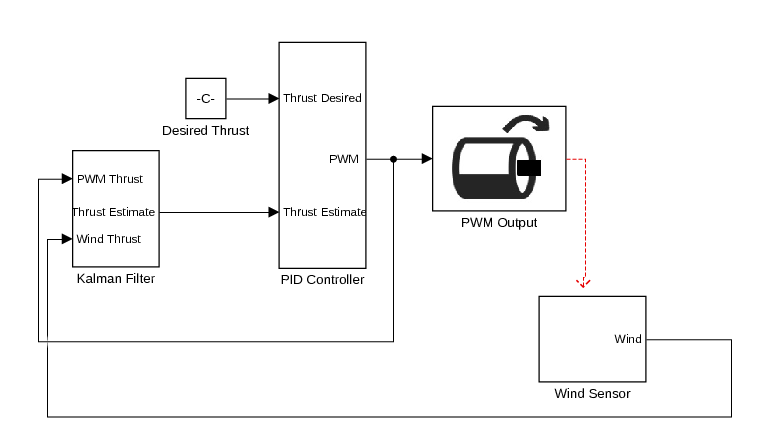
\includegraphics[width=\textwidth / 2]{images/block_diagram.png}
		\caption{Block Diagram}
		\label{block_diagram}
	\end{figure}
	\begin{thebibliography}{99}
		\bibitem{mahoney1} Mahoney 2012
		\bibitem{rcb} https://www.rcbenchmark.com/dynamometer-series-1580/
		\bibitem{md} https://moderndevice.com/product/wind-sensor-rev-p/
		\bibitem{hot_wire} Extended Applications of the Hot‐Wire Anemometer, Stanley Corrsin,Review of Scientific Instruments 1947 18:7, 469-471 
		\bibitem{awan} A. U. Awan, J. Park and H. J. Kim, "Thrust estimation of quadrotor UAV using adaptive observer," 2011 11th International Conference on Control, Automation and Systems, Gyeonggi-do, 2011, pp. 131-136.
		\bibitem{sydney} N. Sydney, B. Smyth and D. A. Paley, "Dynamic control of autonomous quadrotor flight in an estimated wind field," 52nd IEEE Conference on Decision and Control, Florence, 2013, pp. 3609-3616.
		doi: 10.1109/CDC.2013.6760438
		
	\end{thebibliography}


\end{document}